\documentclass[utf8,compress,aspectratio=169]{beamer}
\usepackage{irbookslide}
\usepackage{irilmenau2}
\usepackage{url}
\usepackage{fontspec} % zahteva paket euenc
\usepackage{xunicode}
\usepackage{xltxtra}
\usepackage{polyglossia}
\usepackage[cache=false]{minted}
\usepackage{xcolor,colortbl}
\usepackage{textcomp}
\usepackage{unicode-math}

\usepackage{minted}
\AtBeginEnvironment{minted}{\dontdofcolorbox}
\def\dontdofcolorbox{\renewcommand\fcolorbox[4][]{##4}}

\usepackage{hyperref}
\hypersetup{pdfstartview=Fit}

\title{Računari i programi}
\subtitle{\tiny{Slajdovi za predmet Osnove programiranja}}
\subject{Osnove programiranja}
\institute{Katedra za informatiku, Fakultet tehničkih nauka, Novi Sad}
\date{2022.}

\begin{document}

% da pygmentize ne uokviruje crvenom bojom nepoznate karaktere
\expandafter\def\csname PY@tok@err\endcsname{}

\frame{\titlepage}

\section{Uvod}

\frame{
  \frametitle{Ciljevi}
  \begin{itemize}
    \item razumevanje uloge hardvera i softvera u računarskom sistemu
    \item upoznavanje sa predmetom izučavanja računarstva i tehnikama koje se koriste
    \item razumevanje osnovnih principa rada modernog računara
    \item razumevanje oblika i svrhe programskih jezika
    \item početak korišćenja Python programskog jezika
  \end{itemize}
}

\frame{
  \frametitle{Univerzalna mašina}
  \begin{itemize}
    \item moderan računar:\\ ,,mašina koja skladišti i manipuliše informacijama pod kontrolom izmenljivog programa``
    \item dva ključna elementa:
    \begin{itemize}
      \item računari su uređaji za manipulisanje informacijama
      \item računari funkcionišu pod kontrolom izmenljivog programa
    \end{itemize}
  \end{itemize}
}

\frame{
  \frametitle{Univerzalna mašina $_2$}
  \begin{itemize}
    \item šta je računarski program?
    \begin{itemize}
      \item detaljan, korak-po-korak skup instrukcija koje govore računaru šta da radi
      \item ako izmenimo program, računar će izvršavati drugačiji skup operacija
      \item mašina ostaje ista, ali se program menja
    \end{itemize}
  \end{itemize}
}

\frame{
  \frametitle{Univerzalna mašina $_3$}
  \begin{itemize}
    \item programi se \myblue{izvršavaju}
    \item svi računari imaju istu moć uz odgovarajuće programiranje, tj. svaki računar može da uradi ono što i bilo koji drugi
    \begin{itemize}
      \item ...u principu
    \end{itemize}
  \end{itemize}
}

\frame{
  \frametitle{Moć programa}
  \begin{itemize}
    \item \myblue{softver} (programi) upravlja \myblue{hardverom} (fizičkom mašinom)
    \item proces kreiranja softvera zove se \myblue{programiranje}
    \item zašto učiti programiranje?
    \begin{itemize}
      \item bazično znanje iz računarstva
      \item poznavanje programiranja pomaže razumevanju mogućnosti i ograničenja računara
    \end{itemize}
  \end{itemize}
}

\frame{
  \frametitle{Moć programa $_2$}
  \begin{itemize}
    \item zašto učiti programiranje?
    \begin{itemize}
      \item pomaže čoveku da bude bolji korisnik računara
      \item može biti zabavno
      \item oblik izražavanja
      \item pomaže razvoju veštine rešavanja složenih problema, naročito kod analize složenih sistema i njihovog rastavljanja na manje delove
      \item tražena profesija
    \end{itemize}
  \end{itemize}
}

\frame{
  \frametitle{Način razmišljanja}

  Pošalje žena muža programera u prodavnicu...

  \ %

  - Kupi margarin, a ako ima jaja - kupi 10!

  \ %

  Muž ode u radnju, vraća se kući, stavi na sto 10 margarina i kaže: Ima jaja.
}

\frame{
  \frametitle{Šta je računarstvo?}
  \begin{itemize}
    \item nije izučavanje računara:\\
       ,,Computers are to computer science what telescopes are to astronomy`` \\-- E. Dijkstra
    \item $\rightarrow$ kakve procese možemo opisati?
    \item $\rightarrow$ šta se može izračunati?
  \end{itemize}
}

\frame{
  \frametitle{Šta je računarstvo? $_2$}
  \begin{itemize}
    \item dizajn
    \begin{itemize}
      \item način da se dokaže da se neki problem može rešiti je da se napravi rešenje
      \item to se radi razvojem \myblue{algoritma}, korak-po-korak niza instrukcija koje dovode do rešenja
      \item problem -- na ovaj način možemo dokazati da rešenje postoji, ali ne i da ne postoji
    \end{itemize}
  \end{itemize}
}

\frame{
  \frametitle{Šta je računarstvo? $_3$}
  \begin{itemize}
    \item analiza
    \begin{itemize}
      \item analiza je matematički postupak ispitivanja problema i algoritama
      \item neki naizgled jednostavni problemi ne mogu se rešiti algoritmom -- to su \myblue{nerešivi} problemi
      \item problemi mogu biti \myblue{neizračunljivi} ako se njihova rešenja izvršavaju suviše dugo ili koriste previše memorije
    \end{itemize}
  \end{itemize}
}

\frame{
  \frametitle{Šta je računarstvo? $_4$}
  \begin{itemize}
    \item eksperimenti
    \begin{itemize}
      \item neki problemi su suviše komplikovani za analizu
      \item napravi računarski sistem (hw+sw) pa posmatraj njegovo ponašanje
    \end{itemize}
  \end{itemize}
}

\section{Hardver}

\frame{
  \frametitle{Osnove hardvera}
  \begin{itemize}
    \item procesor (\myblue{centralna procesna jedinica}, CPU) je ,,mozak`` računara
    \begin{itemize}
      \item CPU izvršava sve osnovne operacije nad podacima
      \item npr. jednostavne aritmetičke operacije, poređenje brojeva
    \end{itemize}
  \end{itemize}
}

\frame{
  \frametitle{Osnove hardvera $_2$}
  \begin{itemize}
    \item memorija skladišti programe i podatke
    \begin{itemize}
      \item CPU može da direktno pristupi samo podacima u \myblue{RAM} (random access memory)
      \item RAM je brza, ali ne pamti podatke nakog gubitka napajanja
      \item sekundarna memorija trajno pamti podatke, veći kapacitet, sporija -- magnetna, optička, elektronska
    \end{itemize}
  \end{itemize}
}

\frame{
  \frametitle{Osnove hardvera $_3$}
  \begin{itemize}
    \item ulazni uređaji
    \begin{itemize}
      \item podaci se unose u računar putem tastature, miša, itd.
    \end{itemize}
    \item izlazni uređaji
    \begin{itemize}
      \item obrađeni podaci se prikazuju čoveku putem monitora, štampača, itd.
    \end{itemize}
  \end{itemize}
}

\frame{
  \frametitle{Osnove hardvera $_4$}
  \begin{itemize}
    \item ciklus \myblue{dobavi-i-izvrši}
    \begin{itemize}
      \item pročitaj instrukciju iz RAM
      \item dekodiraj instrukciju -- da se odredi šta ona predstavlja
      \item izvrši potrebnu akciju
      \item naredna instrukcija dobavljena, dekodirana, izvršena
      \item ...ponavljaj
    \end{itemize}
  \end{itemize}
}

\section{Programski jezici}

\frame{
  \frametitle{Programski jezici}
  \begin{itemize}
    \item prirodni jezik može biti neprecizan i dvosmislen kada se opisuju složeni algoritmi
    \begin{itemize}
      \item programi koji su pisani precizno i nedvosmisleno koriste \myblue{programske jezike}
      \item svaka struktura u programskom jeziku ima precizan oblik -- \myblue{sintaksu}
      \item svaka struktura u programskom jeziku ima precizno značenje -- \myblue{semantiku}
    \end{itemize}
  \end{itemize}
}

\frame{
  \frametitle{Programski jezici $_2$}
  \begin{itemize}
    \item programski jezik je kao \myblue{kôd} za zapisivanje instrukcija
    \begin{itemize}
      \item programeri ga obično zovu \myblue{programski kôd}
      \item pisanje algoritama na programskom jeziku se zove \myblue{kodiranje}
    \end{itemize}
  \end{itemize}
}

\frame{
  \frametitle{Programski jezici $_3$}
  \begin{itemize}
    \item programski jezici \myblue{visokog nivoa}
    \begin{itemize}
      \item dizajnirani tako da ih razume i koristi čovek
    \end{itemize}
    \item programski jezici \myblue{niskog nivoa}
    \begin{itemize}
      \item hardver može da razume samo mašinski jezik
    \end{itemize}
  \end{itemize}
}

\frame{
  \frametitle{Programski jezici $_4$}
  \begin{itemize}
    \item saberi dva broja
    \begin{itemize}
      \item učitaj broj iz memorijske lokacije br. 2500 u CPU
      \item učitaj broj iz memorijske lokacije br. 2501 u CPU
      \item saberi dva broja u CPU
      \item uskladišti rezultat u lokaciju br. 2502
    \end{itemize}
    \item ovakve instrukcije niskog nivoa su predstavljene binarnim kodom \{0,1\}
  \end{itemize}
}

\begin{frame}[fragile]
  \frametitle{Primer mašinskog programa -- unos jednog znaka sa tastature}
  \begin{itemize}
    \item za procesor Motorola 6800
  \end{itemize}
  \begin{center}
    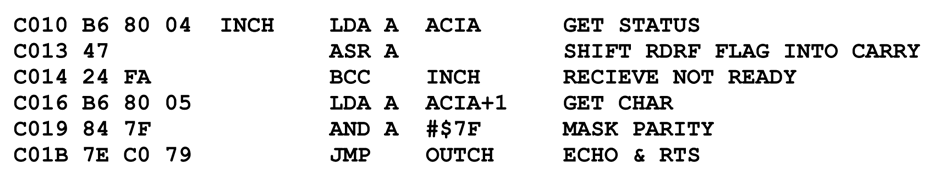
\includegraphics[width=12cm]{motorola-6800-example.png}
  \end{center}
\end{frame}

\begin{frame}[fragile]
  \frametitle{Real programmers code in binary?}
  \begin{center}
    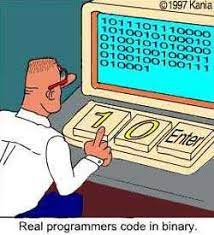
\includegraphics[width=8cm]{real-programmers.jpg}
  \end{center}
\end{frame}

\frame{
  \frametitle{Programski jezici $_5$}
  \begin{itemize}
    \item na jeziku visokog nivoa:\\
      \texttt{a, b = input(), input()} \\
      \texttt{c = a + b}
    \item ovo se mora prevesti na mašiski jezik koga računar može da izvrši
    \item \myblue{kompajleri} (prevodioci) prevode program sa jezika visokog nivoa na mašinski jezik nekog računara
  \end{itemize}
}

\frame{
  \frametitle{Programski jezici $_6$}
  \begin{itemize}
    \item \myblue{interpreteri} simuliraju računar koji razume jezik visokog nivoa
    \item izvorni program se ne prevodi na mašinski jezik odjednom
    \item interpreter analizira i izvršava izvorni program instrukciju po instrukciju
  \end{itemize}
}

\frame{
  \frametitle{Programski jezici $_7$}
  \begin{itemize}
    \item \myblue{kompajleri} vs \myblue{interpreteri}
    \begin{itemize}
      \item jednom prevedeni program se može kasnije izvršavati bez izvornog koda i kompajlera
      \item za interpretirani program svaki put je potreban izvorni kod i interpreter
      \item kompajlirani programi se (u principu) brže izvršavaju jer se prevođenje obavlja samo jednom
    \end{itemize}
  \end{itemize}
}

\frame{
  \frametitle{Programski jezici $_8$}
  \begin{itemize}
    \item \myblue{kompajleri} vs \myblue{interpreteri}
    \begin{itemize}
      \item interpreterski jezici su fleksibilniji jer se mogu pisati i izvršavati interaktivno (naredbu po naredbu)
      \item interpretirani programi su \myblue{prenosivi} -- isti program se može izvršavati na različitim računarima, dok postoji interpreter
    \end{itemize}
  \end{itemize}
}

\section{Python}

\begin{frame}[fragile,shrink=15]
\frametitle{Python}
\begin{itemize}
  \item kada se pokrene Python, vidi se nešto kao:
\end{itemize}
\begin{minted}[fontsize=\small]{text}
Python 3.7.4 (default, Sep  7 2019, 18:27:02)
[Clang 10.0.1 (clang-1001.0.46.4)] on darwin
Type "help", "copyright", "credits" or "license" for more information.
>>>
\end{minted}
\end{frame}


\begin{frame}[fragile]
\frametitle{Python $_2$}
\begin{itemize}
  \item znaci \texttt{>}\texttt{>}\texttt{>} predstavljaju \myblue{prompt} -- Python je spreman da primi naredbu
\end{itemize}
\begin{minted}[fontsize=\small]{python}
>>> print("Hello, world")
Hello, world
>>> print(2+3)
5
>>> print("2+3=", 2+3)
2+3= 5
>>>
\end{minted}
\end{frame}

\begin{frame}[fragile]
\frametitle{Python $_3$}
\begin{itemize}
  \item često nam je potrebno da izvršimo nekoliko naredbi odjednom da bismo rešili neki problem
  \item jedan način da to uradimo je da napravimo \myblue{funkciju}:
\end{itemize}
\begin{minted}[fontsize=\small]{python}
>>> def zdravo():
        print("Zdravo")
        print("Kako si?")
\end{minted}
\end{frame}

\begin{frame}[fragile]
\frametitle{Python $_4$}
\begin{minted}[fontsize=\small]{python}
>>> def zdravo():
        print("Zdravo")
        print("Kako si?")

>>>
\end{minted}
\begin{itemize}
  \item prva linija kaže da definišemo funkciju koja se zove \texttt{zdravo}
  \item naredne linije su uvučene da pokažu da su deo funkcije \texttt{zdravo}
  \item prazan red (pritisnut enter dva puta) kaže Pythonu da je definicija završena
\end{itemize}
\end{frame}

\begin{frame}[fragile]
\frametitle{Python $_5$}
\begin{minted}[fontsize=\small]{python}
>>> def zdravo():
        print("Zdravo")
        print("Kako si?")

>>>
\end{minted}
\begin{itemize}
  \item ništa se do sada nije desilo!
  \item definisali smo funkciju ali nismo rekli Pythonu da je izvrši
  \item funkcija se \myblue{poziva} po imenu:
\end{itemize}
\begin{minted}[fontsize=\small]{python}
>>> zdravo()
Zdravo
Kako si?
>>>
\end{minted}
\end{frame}

\begin{frame}[fragile]
\frametitle{Python $_6$}
\begin{itemize}
  \item čemu služe zagrade?
  \item funkcije mogu zavisiti od nekih podataka koje zovemo \myblue{parametri} koje navodimo između ( i )
\end{itemize}
\begin{minted}[fontsize=\small]{python}
>>> def greet(person):
        print("Hello", person)
        print("How are you?")

>>>
\end{minted}
\end{frame}

\begin{frame}[fragile]
\frametitle{Python $_7$}
\begin{minted}[fontsize=\small]{python}
>>> greet("Pera")
Hello Pera
How are you?
>>> greet("Mika")
Hello Mika
How are you?
\end{minted}
\begin{itemize}
  \item kada koristimo parametre, rezultat rada funkcije može da zavisi od njih
\end{itemize}
\end{frame}

\begin{frame}[fragile]
\frametitle{Python $_8$}
\begin{itemize}
  \item kada prekinemo Python, funkcije koje smo napravili više ne postoje!
  \item programi se tipično sastoje iz funkcija, \myblue{modula} ili \myblue{skriptova} koji se čuvaju na disku da bi se mogli ponovo koristiti
  \item \myblue{modul} fajl je tekst-fajl napisan u editoru teksta koji sadrži programski kod
  \item \myblue{programersko okruženje} (programming environment) je softver koji pomaže programerima da efikasnije pišu programe
\end{itemize}
\end{frame}

\section{Primer}

\begin{frame}[fragile]
\frametitle{Python $_9$}
\begin{minted}[linenos=false]{python}
# chaos.py
# Ovaj program simulira haotično ponašanje

print("Ovaj program simulira haotično ponašanje")
x = eval(input("Unesite broj između 0 i 1: "))
for i in range(10):
    x = 3.9 * x * (1 - x)
    print(x)
\end{minted}
\begin{itemize}
  \item snimićemo fajl sa ekstenzijom \texttt{.py} da označimo Python program
  \item pokrenućemo program sa \texttt{python chaos.py}
\end{itemize}
\end{frame}

\begin{frame}[fragile]
\frametitle{Python $_{10}$}
\begin{verbatim}
$ python chaos.py
Ovaj program simulira haotično ponašanje
Unesite broj između 0 i 1: 0.5
0.975
0.09506250000000008
0.33549992226562525
0.8694649252590003
0.44263310911310905
0.962165255336889
0.1419727793616139
0.4750843861996143
0.9725789275369049
0.1040097132674683
\end{verbatim}
\end{frame}

\begin{frame}[fragile]
\frametitle{Analiza Python programa}
\begin{minted}[linenos=false]{python}
# chaos.py
# Ovaj program ilustruje haotično ponašanje.
\end{minted}
\begin{itemize}
  \item redovi koji počinju sa \texttt{\#} su \myblue{komentari}
  \item namenjene čoveku, Python ih ignoriše
  \item Python preskače tekst od \texttt{\#} do kraja reda
\end{itemize}
\end{frame}

\begin{frame}[fragile]
\frametitle{Analiza Python programa $_2$}
\begin{minted}[linenos=false]{python}
print("Ovaj program ilustruje haotično ponašanje")
\end{minted}
\begin{itemize}
  \item ovaj red kaže Pythonu da ispiše poruku koja opisuje program
\end{itemize}
\end{frame}

\begin{frame}[fragile]
\frametitle{Analiza Python programa $_3$}
\begin{minted}[linenos=false]{python}
x = eval(input("Unesite broj između 0 i 1: "))
\end{minted}
\begin{itemize}
  \item \texttt{x} je primer \myblue{promenljive}
  \item promenljiva se koristi kako bi se nekom \myblue{imenu} dodelila \myblue{vrednost}
  \item možemo se na tu promenljivu kasnije pozvati po imenu
  \item tekst pod navodnicima se ispisuje, i uneti broj se upisuje u promenljivu \texttt{x}.
\end{itemize}
\end{frame}

\begin{frame}[fragile]
\frametitle{Analiza Python programa $_4$}
\begin{minted}[linenos=false]{python}
for i in range(10):
\end{minted}
\begin{itemize}
  \item \texttt{for} predstavlja \myblue{petlju}
  \item petlja govori Pythonu da komande ponavlja više puta
  \item u ovom primeru, kod koji sledi će se ponoviti 10 puta
\end{itemize}
\end{frame}

\begin{frame}[fragile]
\frametitle{Analiza Python programa $_5$}
\begin{minted}[linenos=false]{python}
  x = 3.9 * x * (1 - x)
  print(x)
\end{minted}
\begin{itemize}
  \item ovi redovi predstavljaju \myblue{telo petlje}
  \item telo petlje je ono što se izvršava više puta
  \item naredbe koje čine telo petlje su uvučene u desno
  \item efekat petlje je kao da smo ove dve naredbe ponovili 10 puta
\end{itemize}
\end{frame}

\begin{frame}[fragile,shrink=30]
\frametitle{Analiza Python programa $_6$}
\begin{itemize}
  \item ovo je ekvivalentno
\end{itemize}
\begin{tabular}{|p{5cm}|p{5cm}|}
\begin{minted}[linenos=false]{python}
for i in range(10):
  x = 3.9 * x * (1 - x)
  print(x)
\end{minted}
&
\begin{minted}[linenos=false]{python}
x = 3.9 * x * (1 - x)
print x
x = 3.9 * x * (1 - x)
print x
x = 3.9 * x * (1 - x)
print x
x = 3.9 * x * (1 - x)
print x
x = 3.9 * x * (1 - x)
print x
x = 3.9 * x * (1 - x)
print x
x = 3.9 * x * (1 - x)
print x
x = 3.9 * x * (1 - x)
print x
x = 3.9 * x * (1 - x)
print x
x = 3.9 * x * (1 - x)
print x
\end{minted}
\end{tabular}
\end{frame}

\begin{frame}[fragile]
\frametitle{Analiza Python programa $_7$}
\begin{minted}[linenos=false]{python}
x = 3.9 * x * (1 - x)
\end{minted}
\begin{itemize}
  \item ovo je naredba \myblue{dodele}
  \item izraz sa desne strane \texttt{=} je matematički izraz
  \item \texttt{*} označava množenje
  \item kada se vrednost na desnoj strani izračuna, \myblue{dodeljuje se} (upisuje se) promenljivoj \texttt{x}
\end{itemize}
\end{frame}

\begin{frame}[fragile]
\frametitle{Analiza Python programa $_8$}
\begin{minted}[linenos=false]{python}
def main():
    print("Ovaj program ilustruje haotično ponašanje")
    x = eval(input("Unesite broj između 0 i 1: "))
    for i in range(10):
        x = 3.9 * x * (1 - x)
        print(x)

main()
\end{minted}
\begin{itemize}
  \item sada smo ceo prethodni program smestili u funkciju \texttt{main}
  \item program sadrži definiciju funkcije i njen poziv
\end{itemize}
\end{frame}

\end{document}